% Options for packages loaded elsewhere
\PassOptionsToPackage{unicode}{hyperref}
\PassOptionsToPackage{hyphens}{url}
\PassOptionsToPackage{dvipsnames,svgnames,x11names}{xcolor}
%
\documentclass[
  12pt,
  a4paper,
  DIV=11,
  numbers=noendperiod]{scrartcl}

\usepackage{amsmath,amssymb}
\usepackage{iftex}
\ifPDFTeX
  \usepackage[T1]{fontenc}
  \usepackage[utf8]{inputenc}
  \usepackage{textcomp} % provide euro and other symbols
\else % if luatex or xetex
  \usepackage{unicode-math}
  \defaultfontfeatures{Scale=MatchLowercase}
  \defaultfontfeatures[\rmfamily]{Ligatures=TeX,Scale=1}
\fi
\usepackage{lmodern}
\ifPDFTeX\else  
    % xetex/luatex font selection
\fi
% Use upquote if available, for straight quotes in verbatim environments
\IfFileExists{upquote.sty}{\usepackage{upquote}}{}
\IfFileExists{microtype.sty}{% use microtype if available
  \usepackage[]{microtype}
  \UseMicrotypeSet[protrusion]{basicmath} % disable protrusion for tt fonts
}{}
\makeatletter
\@ifundefined{KOMAClassName}{% if non-KOMA class
  \IfFileExists{parskip.sty}{%
    \usepackage{parskip}
  }{% else
    \setlength{\parindent}{0pt}
    \setlength{\parskip}{6pt plus 2pt minus 1pt}}
}{% if KOMA class
  \KOMAoptions{parskip=half}}
\makeatother
\usepackage{xcolor}
\usepackage[top=20mm,left=20mm,heightrounded]{geometry}
\setlength{\emergencystretch}{3em} % prevent overfull lines
\setcounter{secnumdepth}{-\maxdimen} % remove section numbering
% Make \paragraph and \subparagraph free-standing
\ifx\paragraph\undefined\else
  \let\oldparagraph\paragraph
  \renewcommand{\paragraph}[1]{\oldparagraph{#1}\mbox{}}
\fi
\ifx\subparagraph\undefined\else
  \let\oldsubparagraph\subparagraph
  \renewcommand{\subparagraph}[1]{\oldsubparagraph{#1}\mbox{}}
\fi

\usepackage{color}
\usepackage{fancyvrb}
\newcommand{\VerbBar}{|}
\newcommand{\VERB}{\Verb[commandchars=\\\{\}]}
\DefineVerbatimEnvironment{Highlighting}{Verbatim}{commandchars=\\\{\}}
% Add ',fontsize=\small' for more characters per line
\usepackage{framed}
\definecolor{shadecolor}{RGB}{241,243,245}
\newenvironment{Shaded}{\begin{snugshade}}{\end{snugshade}}
\newcommand{\AlertTok}[1]{\textcolor[rgb]{0.68,0.00,0.00}{#1}}
\newcommand{\AnnotationTok}[1]{\textcolor[rgb]{0.37,0.37,0.37}{#1}}
\newcommand{\AttributeTok}[1]{\textcolor[rgb]{0.40,0.45,0.13}{#1}}
\newcommand{\BaseNTok}[1]{\textcolor[rgb]{0.68,0.00,0.00}{#1}}
\newcommand{\BuiltInTok}[1]{\textcolor[rgb]{0.00,0.23,0.31}{#1}}
\newcommand{\CharTok}[1]{\textcolor[rgb]{0.13,0.47,0.30}{#1}}
\newcommand{\CommentTok}[1]{\textcolor[rgb]{0.37,0.37,0.37}{#1}}
\newcommand{\CommentVarTok}[1]{\textcolor[rgb]{0.37,0.37,0.37}{\textit{#1}}}
\newcommand{\ConstantTok}[1]{\textcolor[rgb]{0.56,0.35,0.01}{#1}}
\newcommand{\ControlFlowTok}[1]{\textcolor[rgb]{0.00,0.23,0.31}{#1}}
\newcommand{\DataTypeTok}[1]{\textcolor[rgb]{0.68,0.00,0.00}{#1}}
\newcommand{\DecValTok}[1]{\textcolor[rgb]{0.68,0.00,0.00}{#1}}
\newcommand{\DocumentationTok}[1]{\textcolor[rgb]{0.37,0.37,0.37}{\textit{#1}}}
\newcommand{\ErrorTok}[1]{\textcolor[rgb]{0.68,0.00,0.00}{#1}}
\newcommand{\ExtensionTok}[1]{\textcolor[rgb]{0.00,0.23,0.31}{#1}}
\newcommand{\FloatTok}[1]{\textcolor[rgb]{0.68,0.00,0.00}{#1}}
\newcommand{\FunctionTok}[1]{\textcolor[rgb]{0.28,0.35,0.67}{#1}}
\newcommand{\ImportTok}[1]{\textcolor[rgb]{0.00,0.46,0.62}{#1}}
\newcommand{\InformationTok}[1]{\textcolor[rgb]{0.37,0.37,0.37}{#1}}
\newcommand{\KeywordTok}[1]{\textcolor[rgb]{0.00,0.23,0.31}{#1}}
\newcommand{\NormalTok}[1]{\textcolor[rgb]{0.00,0.23,0.31}{#1}}
\newcommand{\OperatorTok}[1]{\textcolor[rgb]{0.37,0.37,0.37}{#1}}
\newcommand{\OtherTok}[1]{\textcolor[rgb]{0.00,0.23,0.31}{#1}}
\newcommand{\PreprocessorTok}[1]{\textcolor[rgb]{0.68,0.00,0.00}{#1}}
\newcommand{\RegionMarkerTok}[1]{\textcolor[rgb]{0.00,0.23,0.31}{#1}}
\newcommand{\SpecialCharTok}[1]{\textcolor[rgb]{0.37,0.37,0.37}{#1}}
\newcommand{\SpecialStringTok}[1]{\textcolor[rgb]{0.13,0.47,0.30}{#1}}
\newcommand{\StringTok}[1]{\textcolor[rgb]{0.13,0.47,0.30}{#1}}
\newcommand{\VariableTok}[1]{\textcolor[rgb]{0.07,0.07,0.07}{#1}}
\newcommand{\VerbatimStringTok}[1]{\textcolor[rgb]{0.13,0.47,0.30}{#1}}
\newcommand{\WarningTok}[1]{\textcolor[rgb]{0.37,0.37,0.37}{\textit{#1}}}

\providecommand{\tightlist}{%
  \setlength{\itemsep}{0pt}\setlength{\parskip}{0pt}}\usepackage{longtable,booktabs,array}
\usepackage{calc} % for calculating minipage widths
% Correct order of tables after \paragraph or \subparagraph
\usepackage{etoolbox}
\makeatletter
\patchcmd\longtable{\par}{\if@noskipsec\mbox{}\fi\par}{}{}
\makeatother
% Allow footnotes in longtable head/foot
\IfFileExists{footnotehyper.sty}{\usepackage{footnotehyper}}{\usepackage{footnote}}
\makesavenoteenv{longtable}
\usepackage{graphicx}
\makeatletter
\def\maxwidth{\ifdim\Gin@nat@width>\linewidth\linewidth\else\Gin@nat@width\fi}
\def\maxheight{\ifdim\Gin@nat@height>\textheight\textheight\else\Gin@nat@height\fi}
\makeatother
% Scale images if necessary, so that they will not overflow the page
% margins by default, and it is still possible to overwrite the defaults
% using explicit options in \includegraphics[width, height, ...]{}
\setkeys{Gin}{width=\maxwidth,height=\maxheight,keepaspectratio}
% Set default figure placement to htbp
\makeatletter
\def\fps@figure{htbp}
\makeatother

\KOMAoption{captions}{tableheading}
\usepackage{cancel}
\makeatletter
\@ifpackageloaded{caption}{}{\usepackage{caption}}
\AtBeginDocument{%
\ifdefined\contentsname
  \renewcommand*\contentsname{Table of contents}
\else
  \newcommand\contentsname{Table of contents}
\fi
\ifdefined\listfigurename
  \renewcommand*\listfigurename{List of Figures}
\else
  \newcommand\listfigurename{List of Figures}
\fi
\ifdefined\listtablename
  \renewcommand*\listtablename{List of Tables}
\else
  \newcommand\listtablename{List of Tables}
\fi
\ifdefined\figurename
  \renewcommand*\figurename{Figure}
\else
  \newcommand\figurename{Figure}
\fi
\ifdefined\tablename
  \renewcommand*\tablename{Table}
\else
  \newcommand\tablename{Table}
\fi
}
\@ifpackageloaded{float}{}{\usepackage{float}}
\floatstyle{ruled}
\@ifundefined{c@chapter}{\newfloat{codelisting}{h}{lop}}{\newfloat{codelisting}{h}{lop}[chapter]}
\floatname{codelisting}{Listing}
\newcommand*\listoflistings{\listof{codelisting}{List of Listings}}
\makeatother
\makeatletter
\makeatother
\makeatletter
\@ifpackageloaded{caption}{}{\usepackage{caption}}
\@ifpackageloaded{subcaption}{}{\usepackage{subcaption}}
\makeatother
\ifLuaTeX
  \usepackage{selnolig}  % disable illegal ligatures
\fi
\usepackage{bookmark}

\IfFileExists{xurl.sty}{\usepackage{xurl}}{} % add URL line breaks if available
\urlstyle{same} % disable monospaced font for URLs
\hypersetup{
  pdftitle={OBLIGATORISK INNLEVERING 2, STA-1001 2024},
  colorlinks=true,
  linkcolor={blue},
  filecolor={Maroon},
  citecolor={Blue},
  urlcolor={Blue},
  pdfcreator={LaTeX via pandoc}}

\title{OBLIGATORISK INNLEVERING 2, STA-1001 2024}
\author{}
\date{12-03-2024}

\begin{document}
\maketitle
\begin{abstract}
\hfill\break
\hfill\break
\hfill\break
\hfill\break
\hfill\break
\hfill\break
\hfill\break
\hfill\break
\hfill\break
\hfill\break
\hfill\break
\hfill\break
\hfill\break
\hfill\break
\hfill\break
\hfill\break
\hfill\break
\hfill\break
\hfill\break
\hfill\break
\hfill\break
\hfill\break
\hfill\break
\hfill\break
\hfill\break
\hfill\break
\hfill\break
\hfill\break
\hfill\break
\hfill\break
\hfill\break
\end{abstract}

\renewcommand*\contentsname{Innholdsfortegnelse}
{
\hypersetup{linkcolor=black}
\setcounter{tocdepth}{3}
\tableofcontents
}
\newpage

\subsection{OBLIGATORISK INNLEVERING 2, STA-1001
2024}\label{obligatorisk-innlevering-2-sta-1001-2024}

\subsubsection{INNLEVERINGSFRIST TIRSDAG 12/3 KL
23:59}\label{innleveringsfrist-tirsdag-123-kl-2359}

Oppgavene er fra kapittel 4 - 7. Øvinga leveres som pdf i Canvas.

\subsection{1}\label{section}

De stokastiske variablene \(X\) og \(Y\) har simultan
sannsynlighetstetthet \[
f(x,y) = 
\begin{cases}
\frac{1}{2} \sqrt y e^{-xy}, & 0 < x < \infty, \ 1 < y < 4. \\
0, & \text{ellers}.
\end{cases}
\]

\subsubsection{\texorpdfstring{a) Vis at fordelinga for \(Y\)
(marginalfordeling) har
sannsynlighetstetthet}{a) Vis at fordelinga for Y (marginalfordeling) har sannsynlighetstetthet}}\label{a-vis-at-fordelinga-for-y-marginalfordeling-har-sannsynlighetstetthet}

\[ h(y) = \frac{1}{2\sqrt{y}}, 1 < y < 4. \]

\begin{Shaded}
\begin{Highlighting}[]
\ImportTok{from}\NormalTok{ IPython.display }\ImportTok{import}\NormalTok{ display}
\ImportTok{import}\NormalTok{ sympy }\ImportTok{as}\NormalTok{ sp}
\NormalTok{x, y }\OperatorTok{=}\NormalTok{ sp.symbols(}\StringTok{\textquotesingle{}x y\textquotesingle{}}\NormalTok{)}
\NormalTok{oppgave1a }\OperatorTok{=}\NormalTok{ sp.integrate((}\DecValTok{1}\OperatorTok{/}\DecValTok{2}\NormalTok{)}\OperatorTok{*}\NormalTok{sp.sqrt(y)}\OperatorTok{*}\NormalTok{sp.exp(}\OperatorTok{{-}}\NormalTok{x}\OperatorTok{*}\NormalTok{y), (x, }\DecValTok{0}\NormalTok{, sp.oo))}
\NormalTok{display(oppgave1a)}
\end{Highlighting}
\end{Shaded}

$\displaystyle \begin{cases} \frac{0.5}{\sqrt{y}} & \text{for}\: \left|{\arg{\left(y \right)}}\right| < \frac{\pi}{2} \\\int\limits_{0}^{\infty} 0.5 \sqrt{y} e^{- x y}\, dx & \text{otherwise} \end{cases}$

Utregning

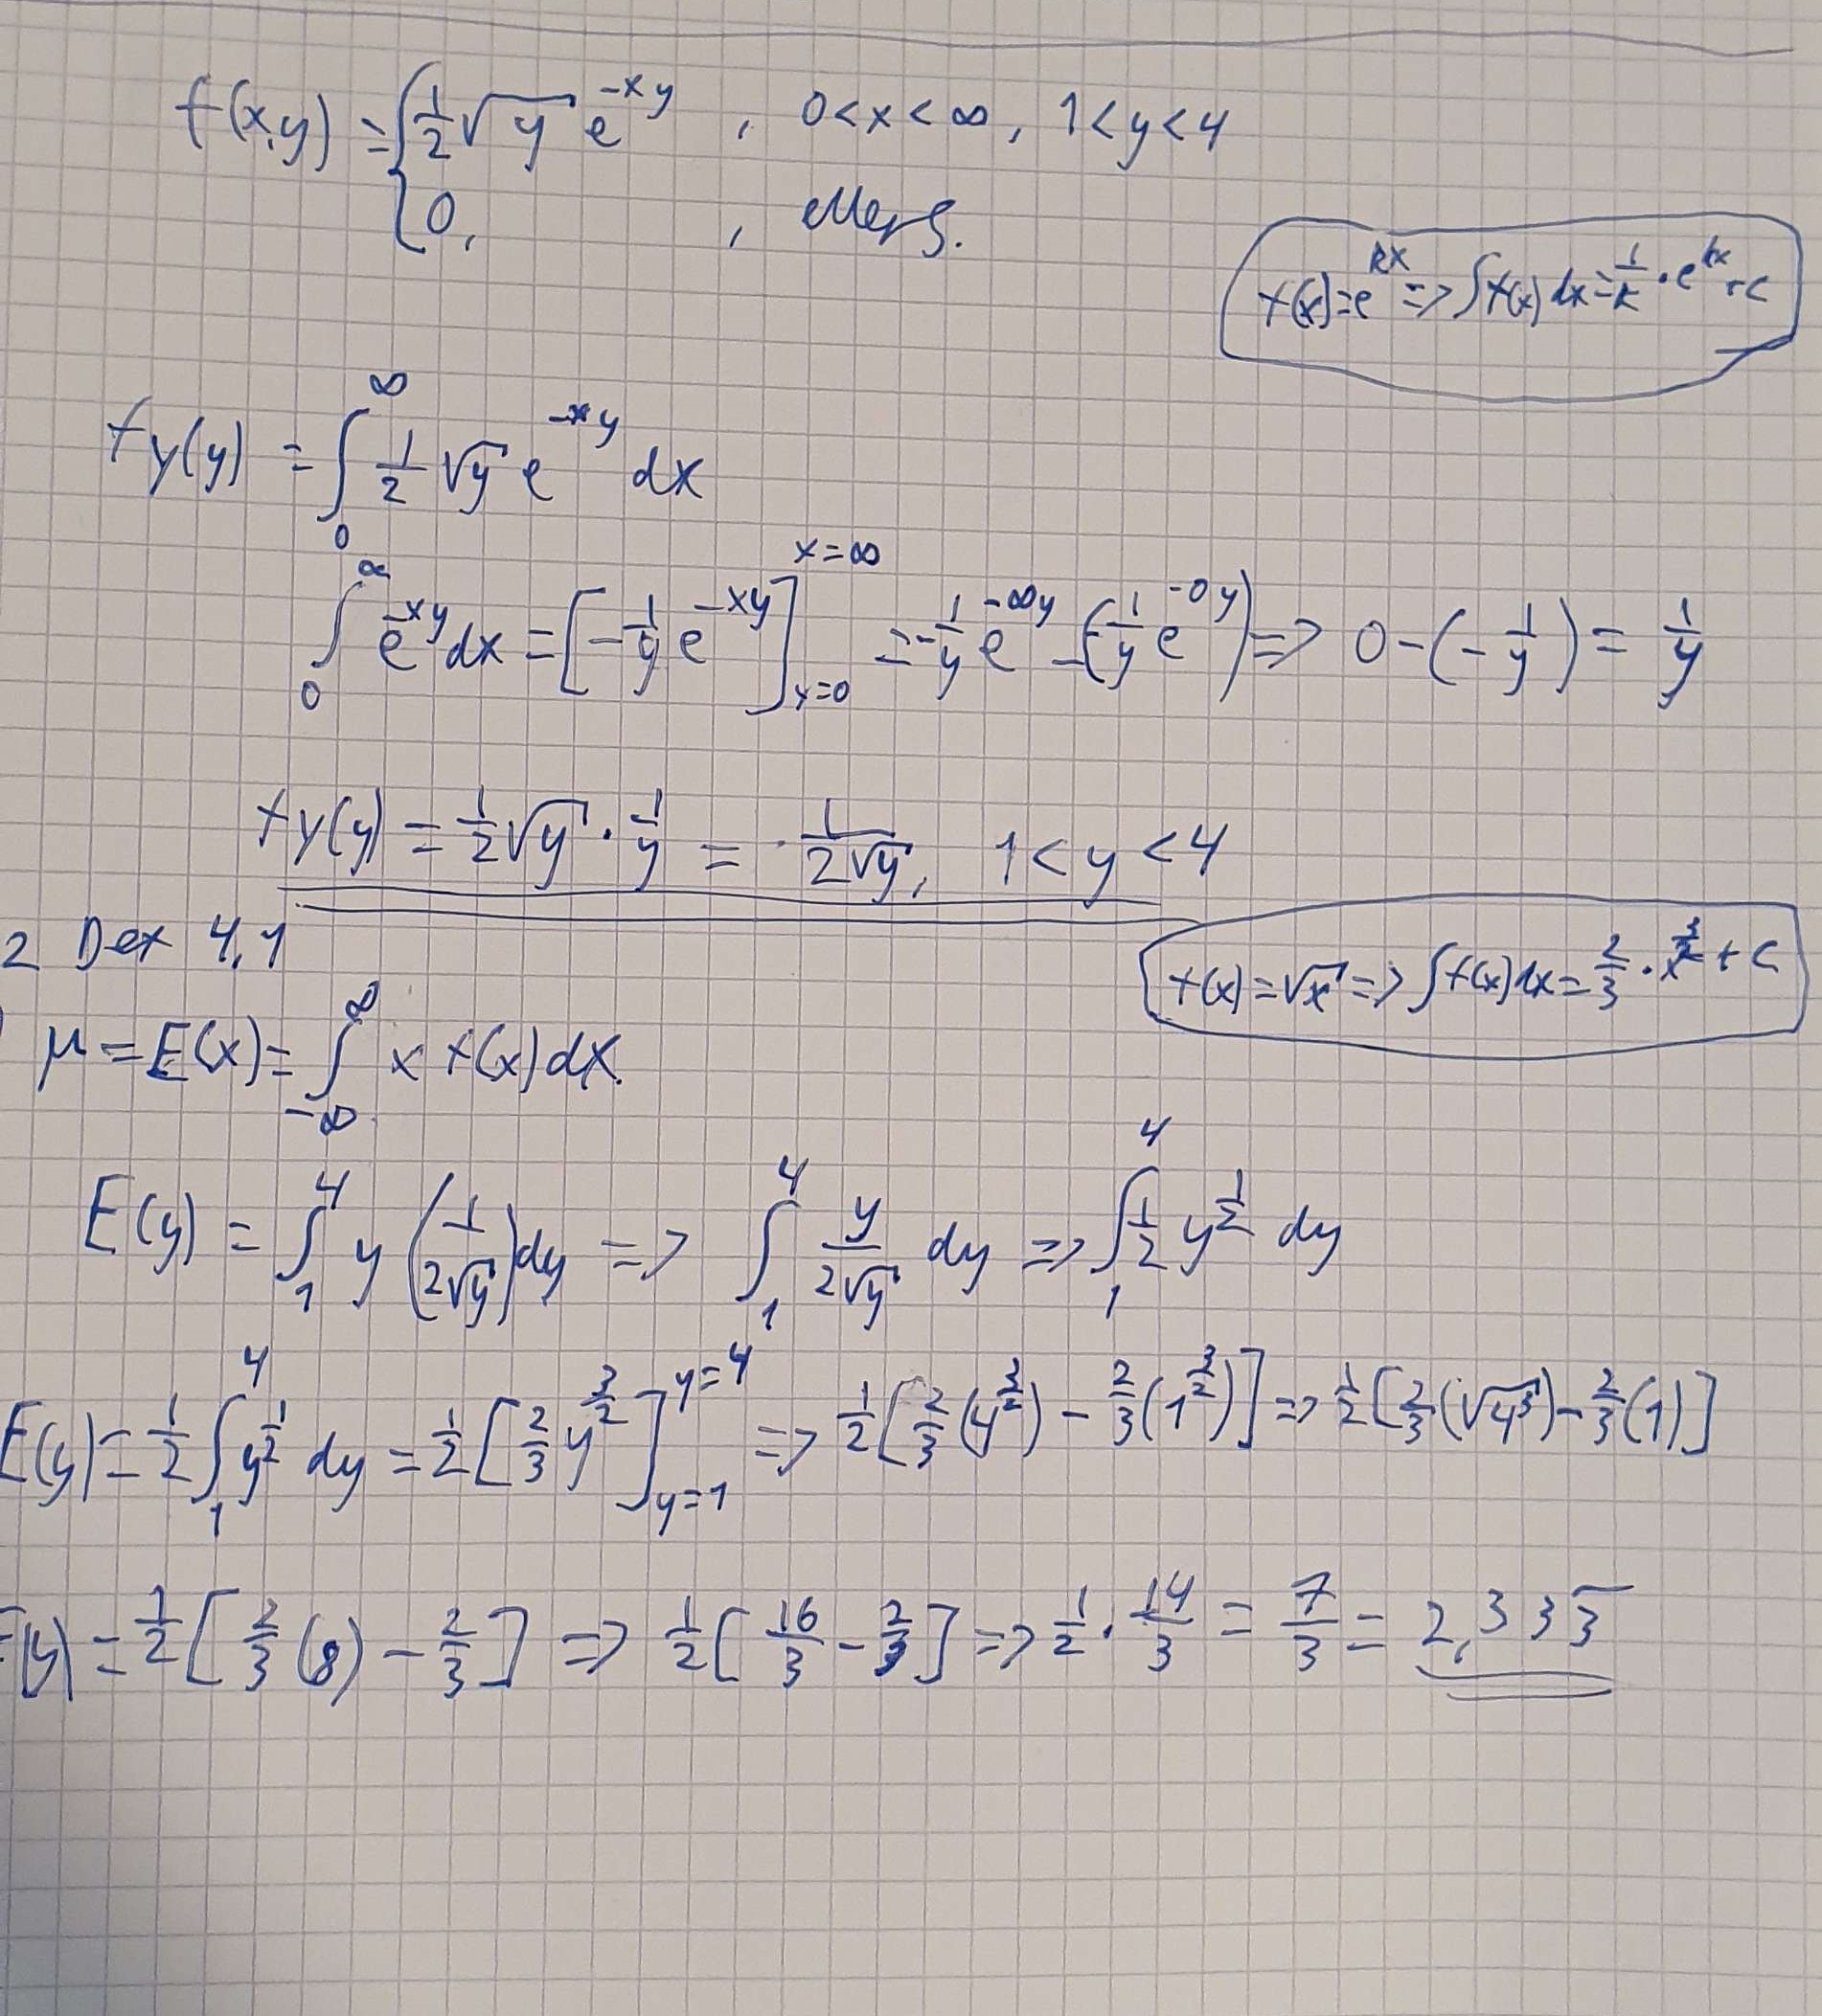
\includegraphics{oblig2_utregning/oppgave1_a.jpg}

\subsubsection{\texorpdfstring{b) Finn forventningsverdi, varians og
standardavvik for
\(Y\).}{b) Finn forventningsverdi, varians og standardavvik for Y.}}\label{b-finn-forventningsverdi-varians-og-standardavvik-for-y.}

\begin{Shaded}
\begin{Highlighting}[]
\CommentTok{\# Beregner E(Y)}
\NormalTok{E\_Y }\OperatorTok{=}\NormalTok{ sp.integrate(y }\OperatorTok{*}\NormalTok{ oppgave1a, (y, }\DecValTok{1}\NormalTok{, }\DecValTok{4}\NormalTok{))}

\CommentTok{\# Beregner E(Y\^{}2)}
\NormalTok{E\_Y2 }\OperatorTok{=}\NormalTok{ sp.integrate(y}\OperatorTok{**}\DecValTok{2} \OperatorTok{*}\NormalTok{ oppgave1a, (y, }\DecValTok{1}\NormalTok{, }\DecValTok{4}\NormalTok{))}

\CommentTok{\# Beregner variansen for Y}
\NormalTok{var }\OperatorTok{=}\NormalTok{ E\_Y2 }\OperatorTok{{-}}\NormalTok{ E\_Y}\OperatorTok{**}\DecValTok{2}

\CommentTok{\# Beregner standardavviket for Y}
\NormalTok{std }\OperatorTok{=}\NormalTok{ sp.sqrt(var)}

\BuiltInTok{print}\NormalTok{(}\SpecialStringTok{f"Forventningsverdien er }\SpecialCharTok{\{}\BuiltInTok{round}\NormalTok{(E\_Y, }\DecValTok{2}\NormalTok{)}\SpecialCharTok{\}}\CharTok{\textbackslash{}n}\SpecialStringTok{Variansen er }\SpecialCharTok{\{}\BuiltInTok{round}\NormalTok{(var, }\DecValTok{2}\NormalTok{)}\SpecialCharTok{\}}\SpecialStringTok{ }\CharTok{\textbackslash{}n}\SpecialStringTok{Standardavviket er }\SpecialCharTok{\{}\BuiltInTok{round}\NormalTok{(std, }\DecValTok{2}\NormalTok{)}\SpecialCharTok{\}}\SpecialStringTok{."}\NormalTok{)}
\end{Highlighting}
\end{Shaded}

\begin{verbatim}
Forventningsverdien er 2.33
Variansen er 0.76 
Standardavviket er 0.87.
\end{verbatim}

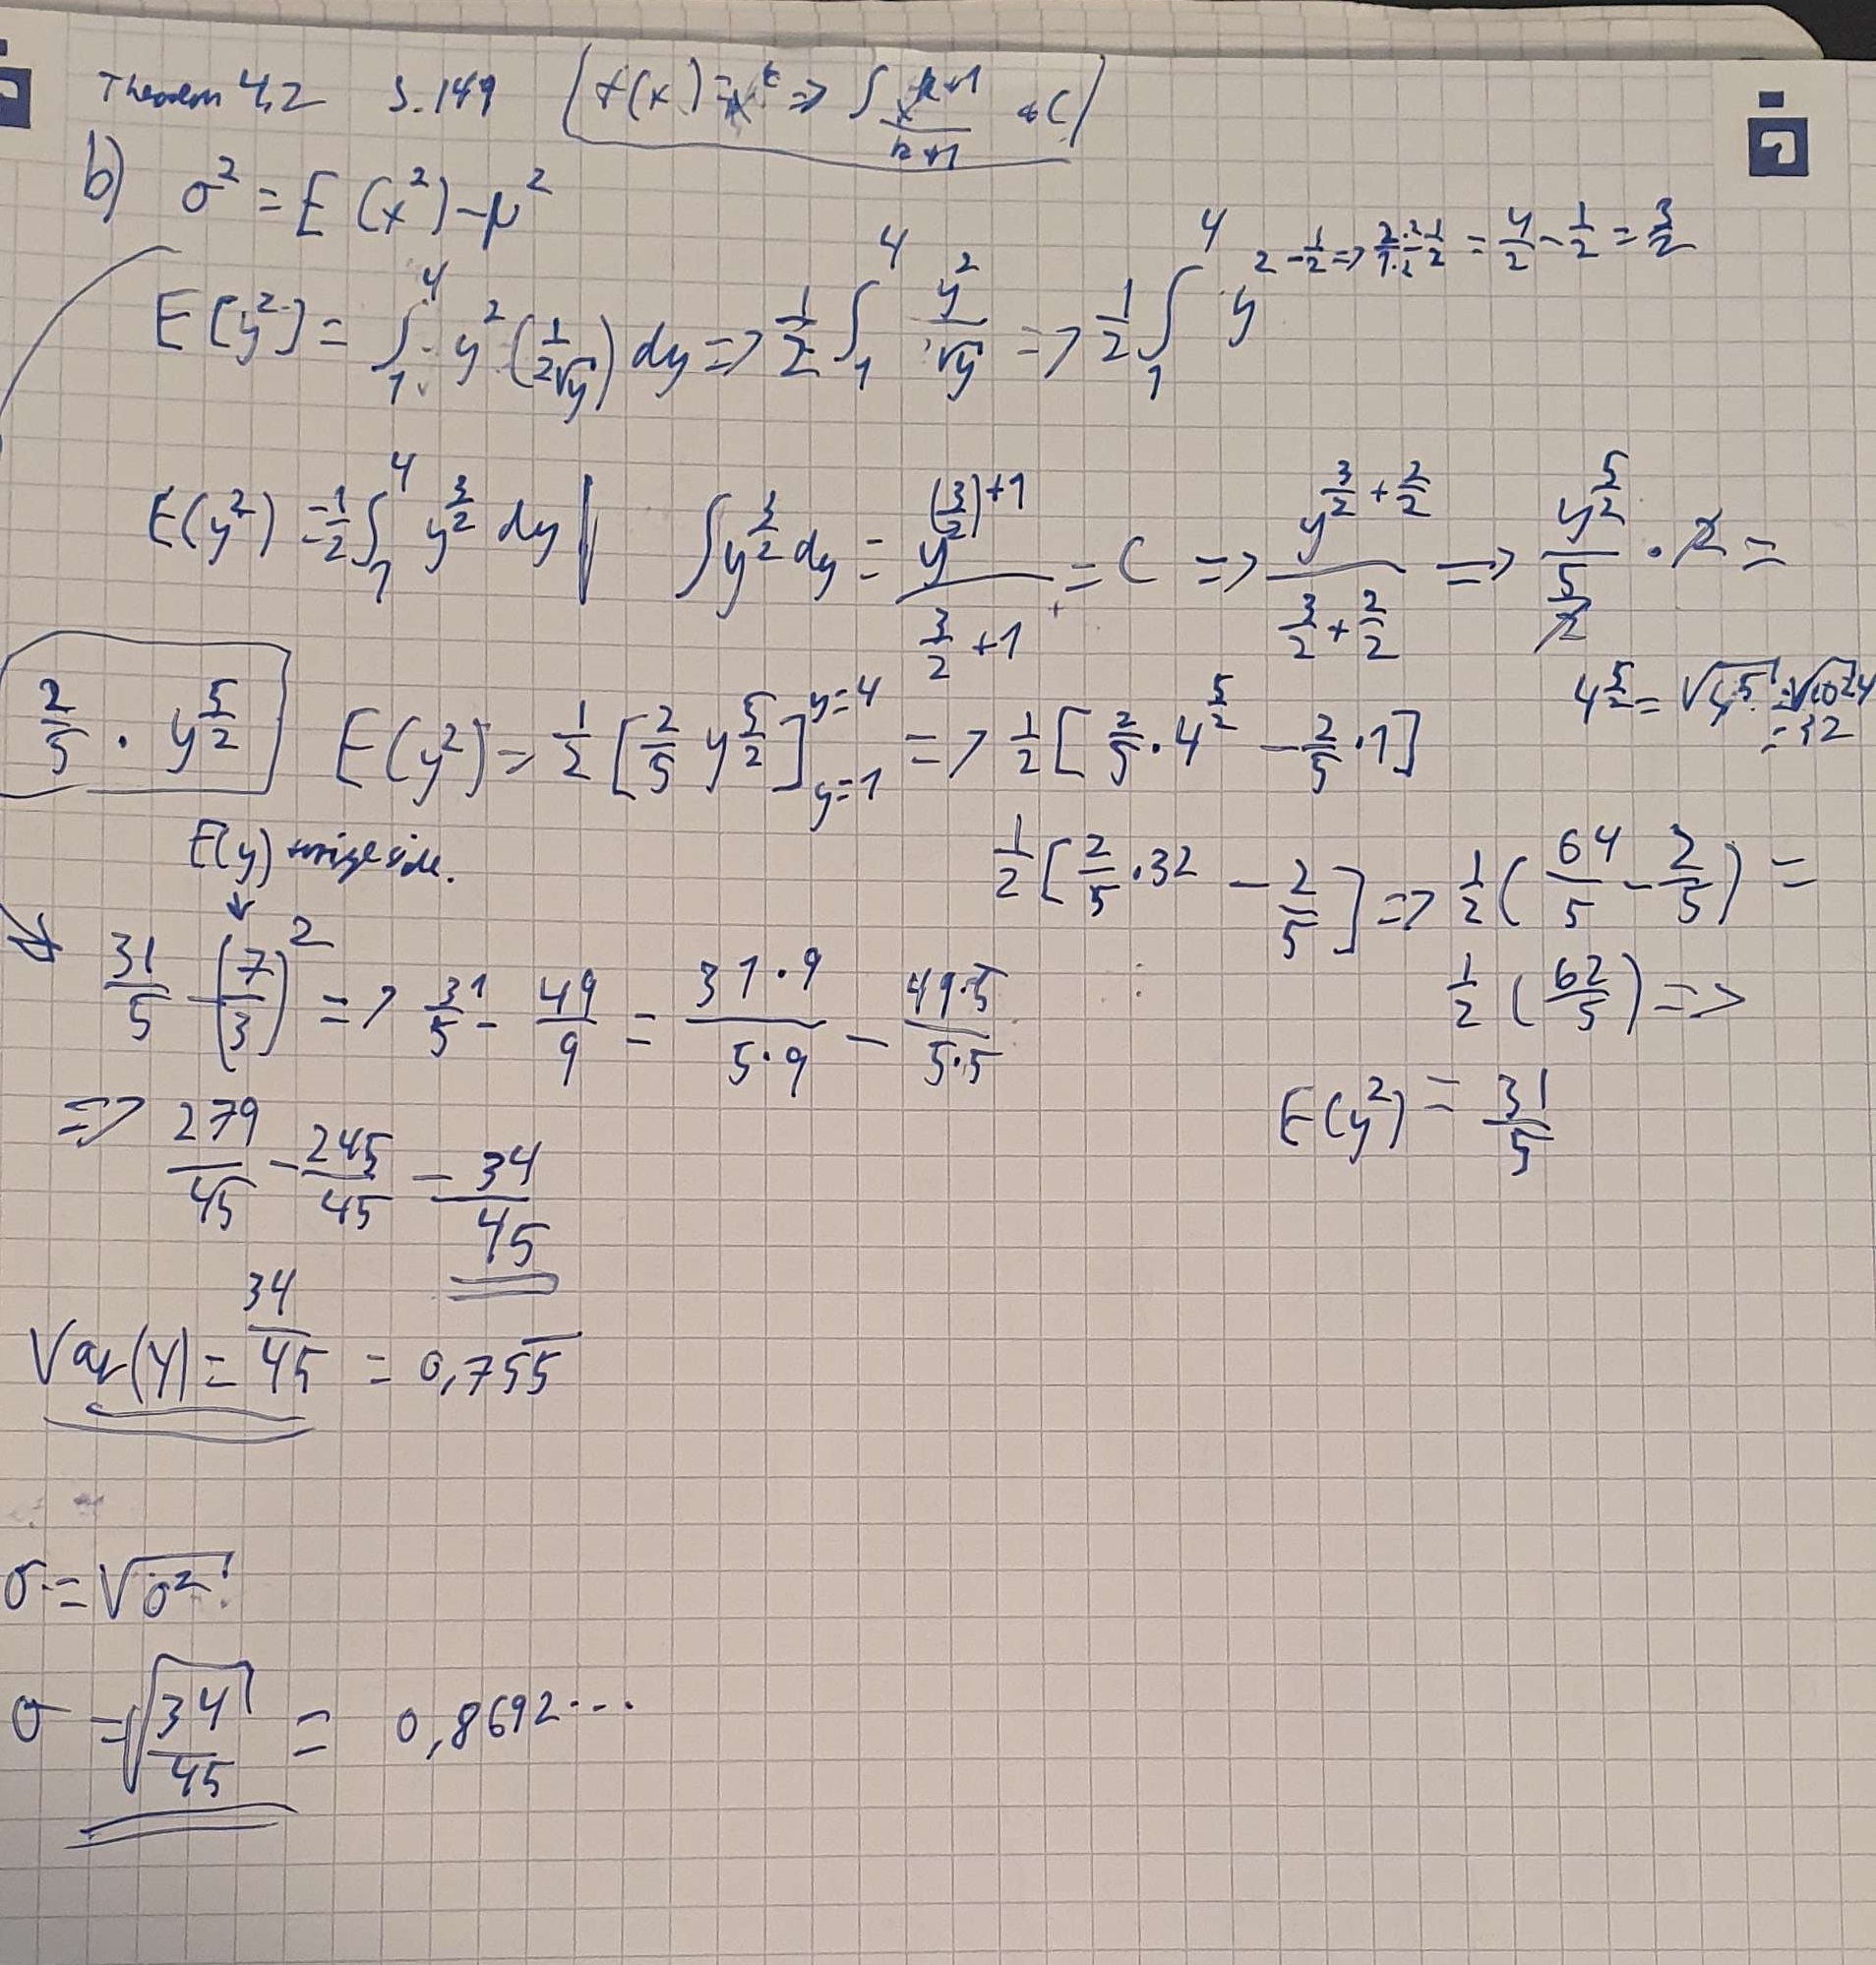
\includegraphics{oblig2_utregning/oppgave1_b.jpg}

\subsubsection{\texorpdfstring{c) Bruk den simultane
sannsynlighetstettheten til å finne \(E(XY)\) og
\(E(X)\).}{c) Bruk den simultane sannsynlighetstettheten til å finne E(XY) og E(X).}}\label{c-bruk-den-simultane-sannsynlighetstettheten-til-uxe5-finne-exy-og-ex.}

Hva blir kovariansen mellom \(X\) og \(Y\)?

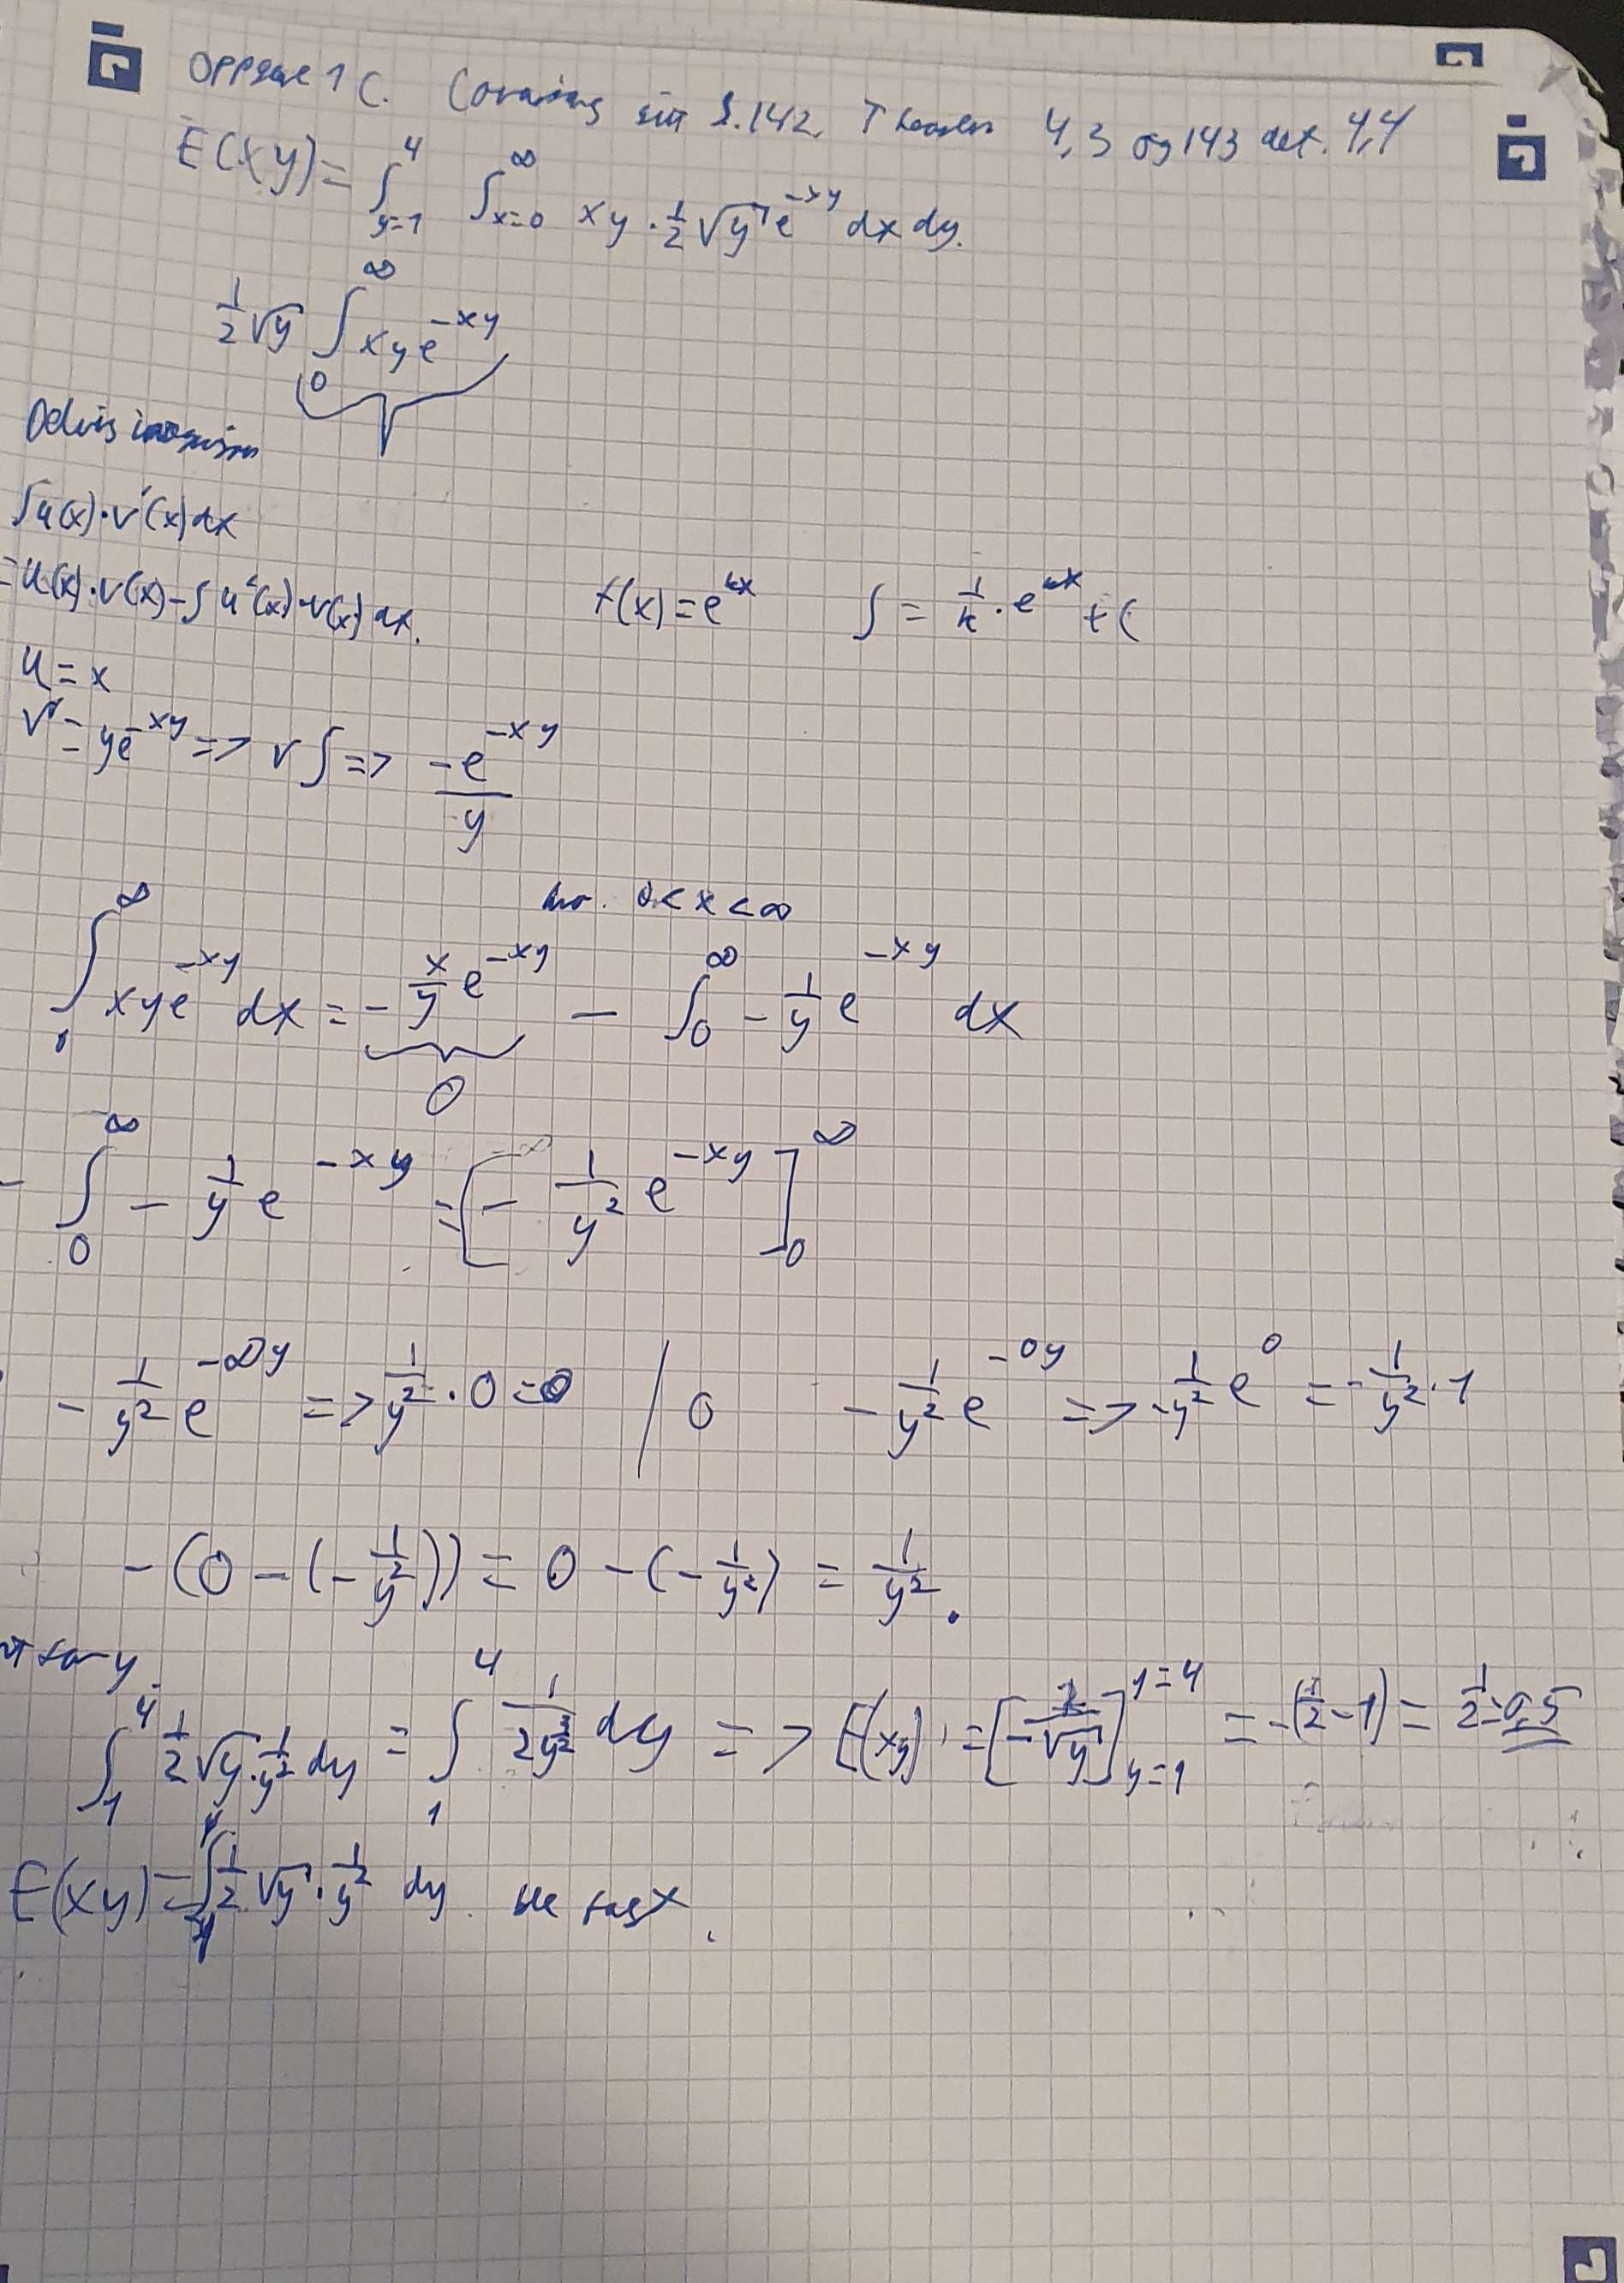
\includegraphics{oblig2_utregning/oppgave1_c_feil.jpg}

Vi er interessert i den stokastiske variabelen \(1/Y\).

\subsubsection{\texorpdfstring{d) Finn forventningsverdi og varians for
\(1/Y\).}{d) Finn forventningsverdi og varians for 1/Y.}}\label{d-finn-forventningsverdi-og-varians-for-1y.}

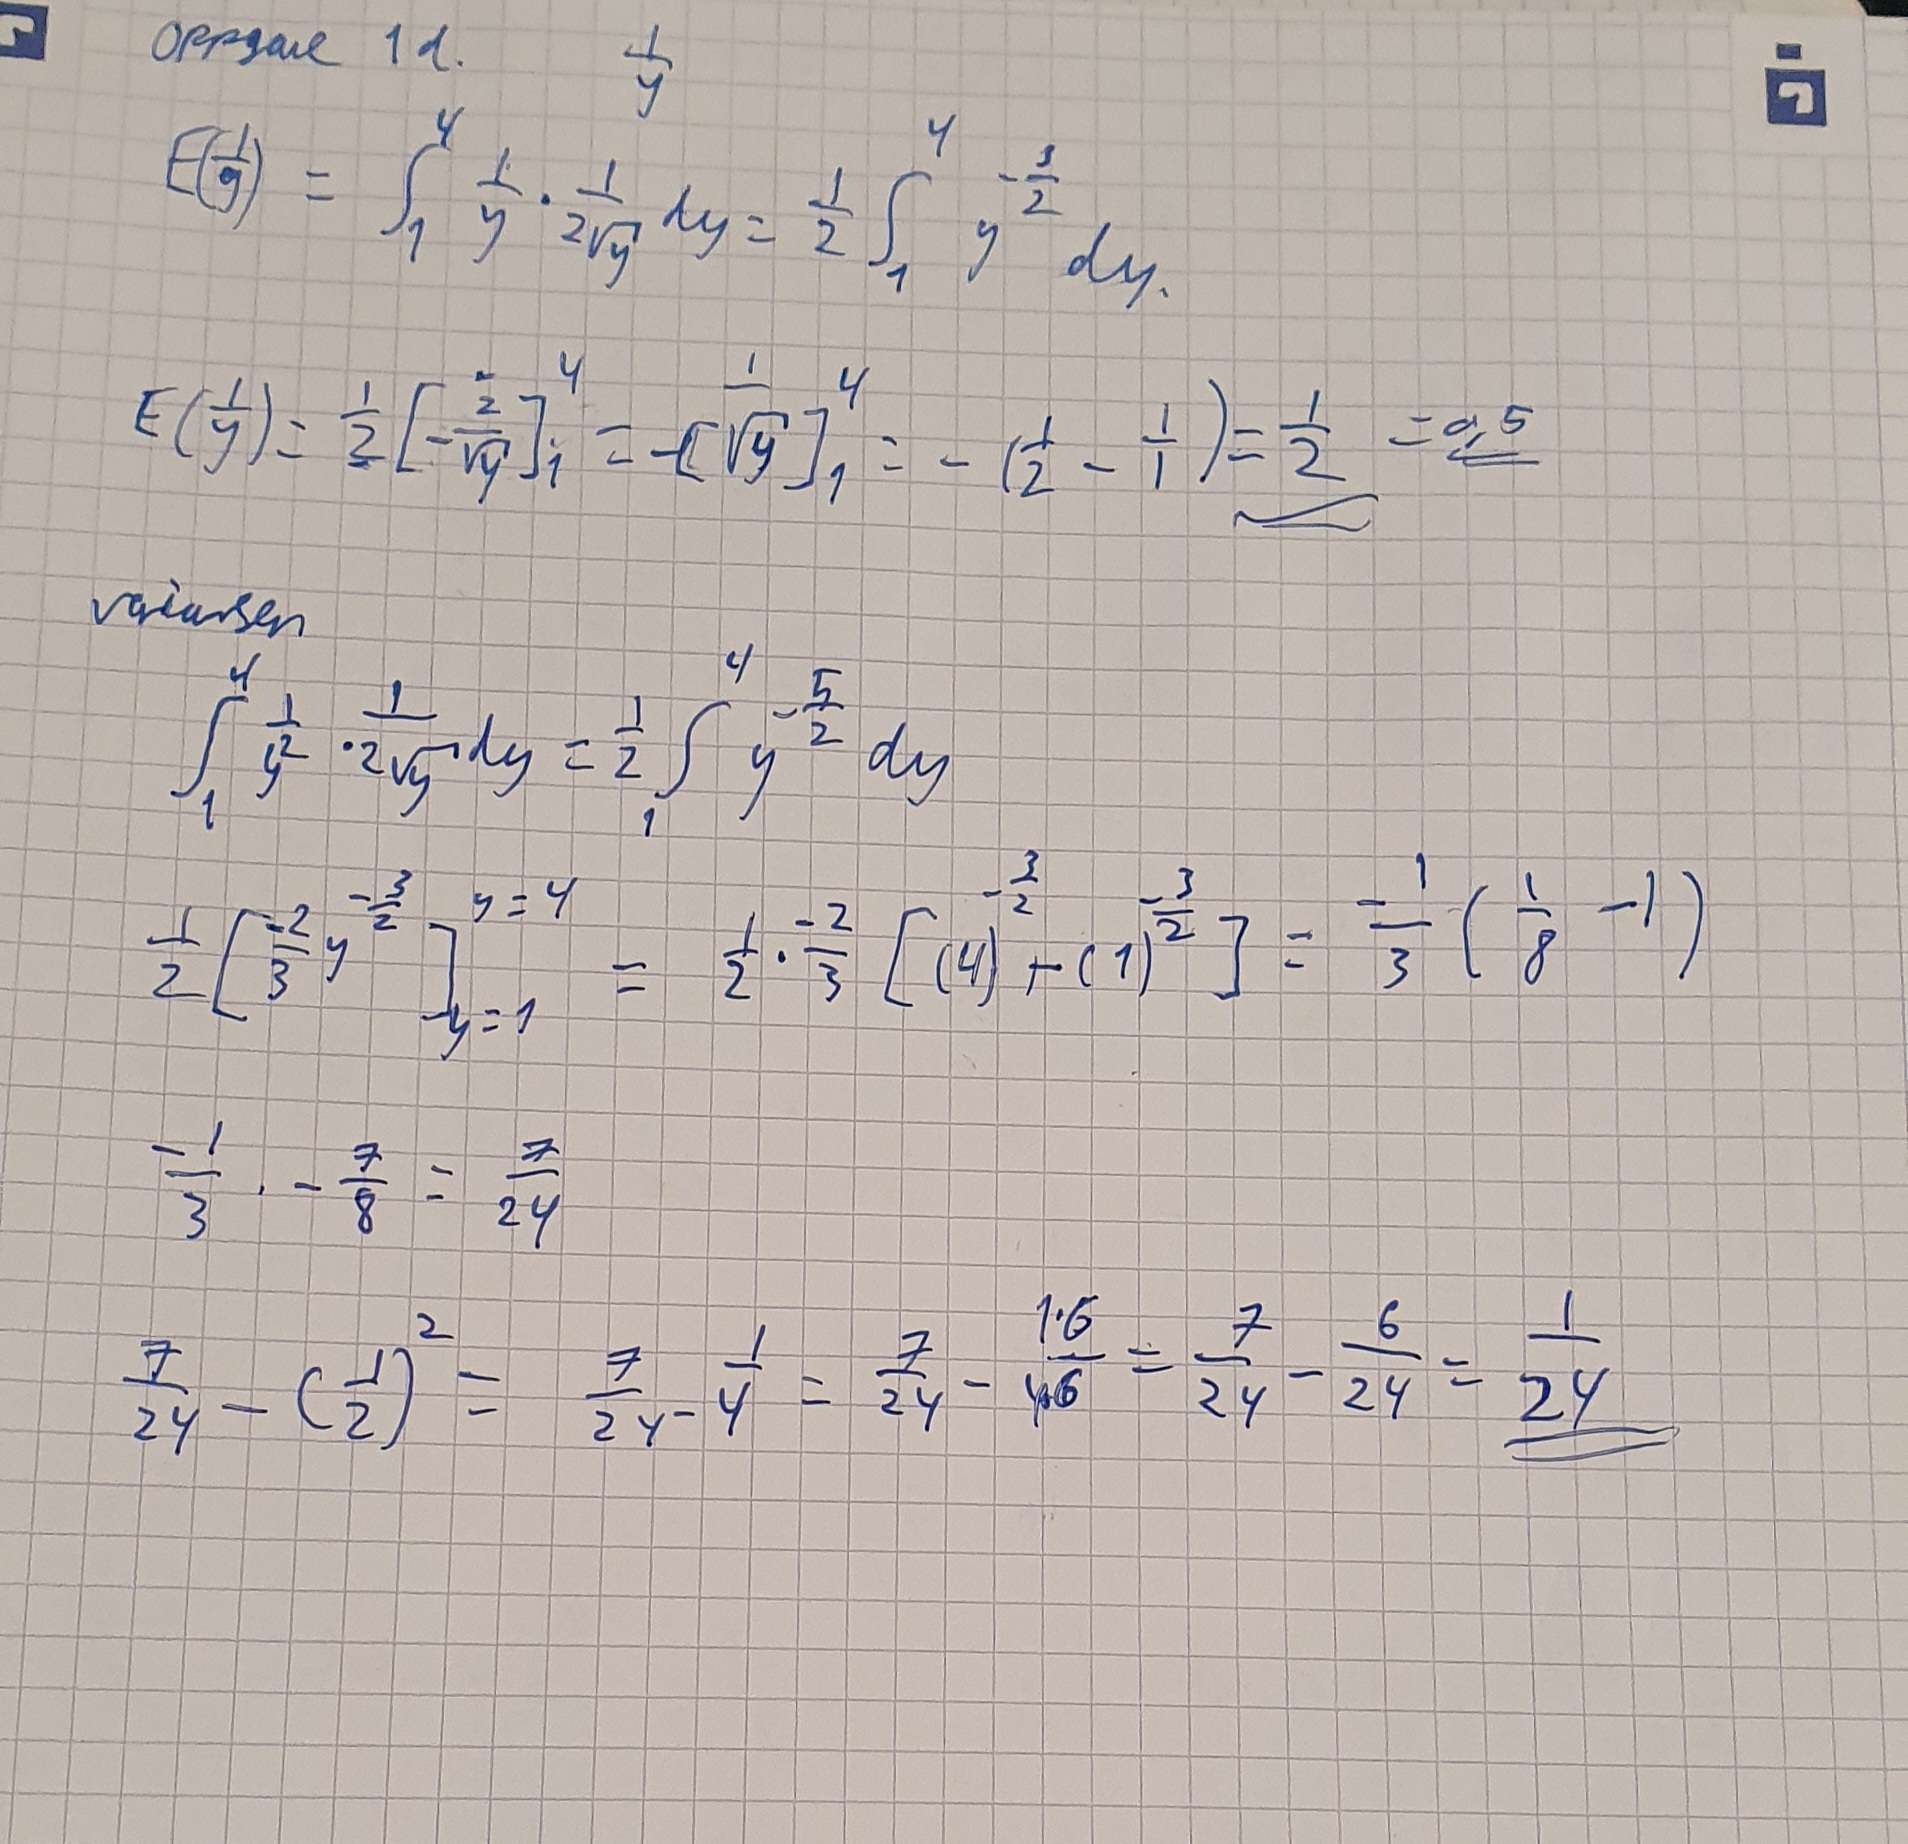
\includegraphics{oblig2_utregning/oppgave1_d.jpg}

\subsection{2}\label{section-1}

Ola samler på spillerkort av fotballspillere (fotballkort). Korta kjøper
han ett og ett av gangen, men de er innpakka så han veit ikke på forhand
om det er et kort han allerede har eller ikke. Vi går ut fra at alle
korta han kjøper er fra en spesiell serie med 10 ulike spillerkort, at
det i hvert kjøp er lik sannsynlighet for alle de 10 ulike spillerkorta,
og at resultata av kortkjøpa er uavhengige. Ola ønsker seg framfor alt
ett bestemt spillerkort (vi kaller han spiller A). La \(X\) være antall
kort han må kjøpe til han får dette kortet.

\paragraph{a1) Forklar hvorfor antakelsene til geometrisk fordeling er
oppfylt.}\label{a1-forklar-hvorfor-antakelsene-til-geometrisk-fordeling-er-oppfylt.}

Det er en konstant sannsynlighet for suksess på hvert forsøk.

Forsøkene er uavhengige av hverandre. utfallet av et kjøp ikke påvirker
utfallet av de neste.

Forsøket blir gjentatt til første suksess

Det er to mulige utfall på hvert forsøk, enten får han kortet eller
ikke.

\paragraph{a2) Hva er sannsynligheten for at han får spillerkortet på
det fjerde
kjøpet?}\label{a2-hva-er-sannsynligheten-for-at-han-fuxe5r-spillerkortet-puxe5-det-fjerde-kjuxf8pet}

\begin{Shaded}
\begin{Highlighting}[]
\NormalTok{sjangse }\OperatorTok{=} \DecValTok{1}\OperatorTok{/}\DecValTok{10}
\NormalTok{x\_num }\OperatorTok{=} \DecValTok{4}
\NormalTok{q\_num }\OperatorTok{=} \DecValTok{1}\OperatorTok{{-}}\NormalTok{sjangse}

\NormalTok{oppgave\_2\_b }\OperatorTok{=}\NormalTok{ sjangse}\OperatorTok{*}\NormalTok{q\_num}\OperatorTok{**}\NormalTok{(x\_num}\OperatorTok{{-}}\DecValTok{1}\NormalTok{)}
\NormalTok{oppgave\_2\_b}
\end{Highlighting}
\end{Shaded}

\begin{verbatim}
0.0729
\end{verbatim}

\paragraph{a3) Dersom han ikke fikk spillerkortet på det første kjøpet,
hva er sannsynligheten for at han skal få det på det
femte?}\label{a3-dersom-han-ikke-fikk-spillerkortet-puxe5-det-fuxf8rste-kjuxf8pet-hva-er-sannsynligheten-for-at-han-skal-fuxe5-det-puxe5-det-femte}

det samme som i a3)

Vi vil se på det som en teoretisk egenskap ved geometrisk fordeling. Vi
antar i b) at antall kjøpte kort følger geometrisk fordeling med
generell sannsynlighet \(p\).

\subsubsection{b) Bruk punktsannsynligheten til geometrisk fordeling til
å vise
at}\label{b-bruk-punktsannsynligheten-til-geometrisk-fordeling-til-uxe5-vise-at}

\[ E(X) = \frac{1}{p} \] Punktssannsynligheten til geometrisk fordeling
er gitt ved \(P(X = k) = (1-p)^{k-1}p\) så forventningsverdien blir
\(E(X) = \sum_{k=1}^{\infty} k(1-p)^{k-1}p\). summen av denne rekken er
\(E(X) = \frac{1}{p}\)

La oss nå tenke oss at det er to spillkort (spiller A og B) Ola spesielt
ønsker seg, og at han kjøper kort til han har fått begge. La \(X\) være
antall kjøp til han får det første av disse spillerkorta, og la \(Y\)
være antall kjøp etter han fikk det første til han får det andre. La
\(T\) være hvor mange kort han må kjøpe totalt for å få disse to
spillerkorta:

\[ T = X + Y \]

\subsubsection{\texorpdfstring{c) Argumentér kort for hvorfor \(X\) og
\(Y\) er uavhengige, og hva som blir fordeling for hver
enkelt.}{c) Argumentér kort for hvorfor X og Y er uavhengige, og hva som blir fordeling for hver enkelt.}}\label{c-argumentuxe9r-kort-for-hvorfor-x-og-y-er-uavhengige-og-hva-som-blir-fordeling-for-hver-enkelt.}

\(X\) og \(Y\) er uavhengige fordi utfallet av kjøpene som leder til det
første ønskede kortet ikke påvirker utfallet av kjøpene etter det første
ønskede kortet er oppnådd. Når Ola starter jakten på det andre kortet,
resettes situasjonen til en ny geometrisk fordeling. Fordelingen av X
starter med p=\(2/10\) fordi det er to kort han ønsker seg, og for Y
starter fordelingen med p=\(1/9\) fordi det nå kun er ett kort han
ønsker seg.

Bruk formler for forventning/varians i geometrisk fordeling til å finne
forventning og varians til \(T\).

\[E(X) = \frac{1}{p}\] \(E(T) = E(X) + E(Y)\) fordi \(T = X + Y\) og
\(X\) og \(Y\) er uavhengige. så
\(E(T) = \frac{1}{p} + \frac{1}{p} = \frac{2}{p}\) setter inn for tall:
\(E(T) = \frac{1}{\frac{2}{2/10}} + \frac{1}{\frac{1}{9}} = 14\)

\[Var(X) = \frac{1-p}{p^2}\]

så \(Var(T) = Var(X) + Var(Y)\) fordi \(X\) og \(Y\) er uavhengige. så
\(Var(T) = \frac{1-p}{p^2} + \frac{1-p}{p^2} = \frac{2(1-p)}{p^2}\).
setter inn for tall:
\(Var(T) = \frac{(1-2/10)}{(2/10)^2} + \frac{1-\frac{1}{9}}{(\frac{1}{9})^2} = 92\)

\subsubsection{d) Argumenter for hva som er fordelinga for antallet kort
i pakka som er med spiller
A?}\label{d-argumenter-for-hva-som-er-fordelinga-for-antallet-kort-i-pakka-som-er-med-spiller-a}

Fordelingen for antall kort i pakka er en binomisk fordeling med n=10 og
p=1/10. Dette er fordi det er 10 kort i pakka og sannsynligheten for at
et kort er spiller A er 1/10.

Hva er sansynligheten for at Ola får minst ett kort med spiller A i
pakka?

\begin{Shaded}
\begin{Highlighting}[]
\ImportTok{from}\NormalTok{ scipy.stats }\ImportTok{import}\NormalTok{ binom}
\NormalTok{n }\OperatorTok{=} \DecValTok{10}
\NormalTok{p }\OperatorTok{=} \DecValTok{1}\OperatorTok{/}\DecValTok{10}
\NormalTok{k }\OperatorTok{=} \DecValTok{1}
\NormalTok{oppgave\_2\_d }\OperatorTok{=} \DecValTok{1} \OperatorTok{{-}}\NormalTok{ binom.cdf(k}\OperatorTok{{-}}\DecValTok{1}\NormalTok{, n, p)}
\NormalTok{oppgave\_2\_d}
\end{Highlighting}
\end{Shaded}

\begin{verbatim}
0.6513215599000001
\end{verbatim}

\subsubsection{e) Hva er forventa antall ulike spillerkort i pakka?
(Hint: Indikatorvariabler for hvert
spillerkort.)}\label{e-hva-er-forventa-antall-ulike-spillerkort-i-pakka-hint-indikatorvariabler-for-hvert-spillerkort.}

Hvis vi går ut ifra at det er 10 kort i pakka så kan vi beregne
forventet antall ulike spillerkort i pakka ved å summere sannsynligheten
for at hvert kort blir valgt minst en gang
\(E(X) = 10 \cdot (1 - (9/10)^{10}) = 10 \cdot (1 - 0.3487) = 6.513\)

\clearpage

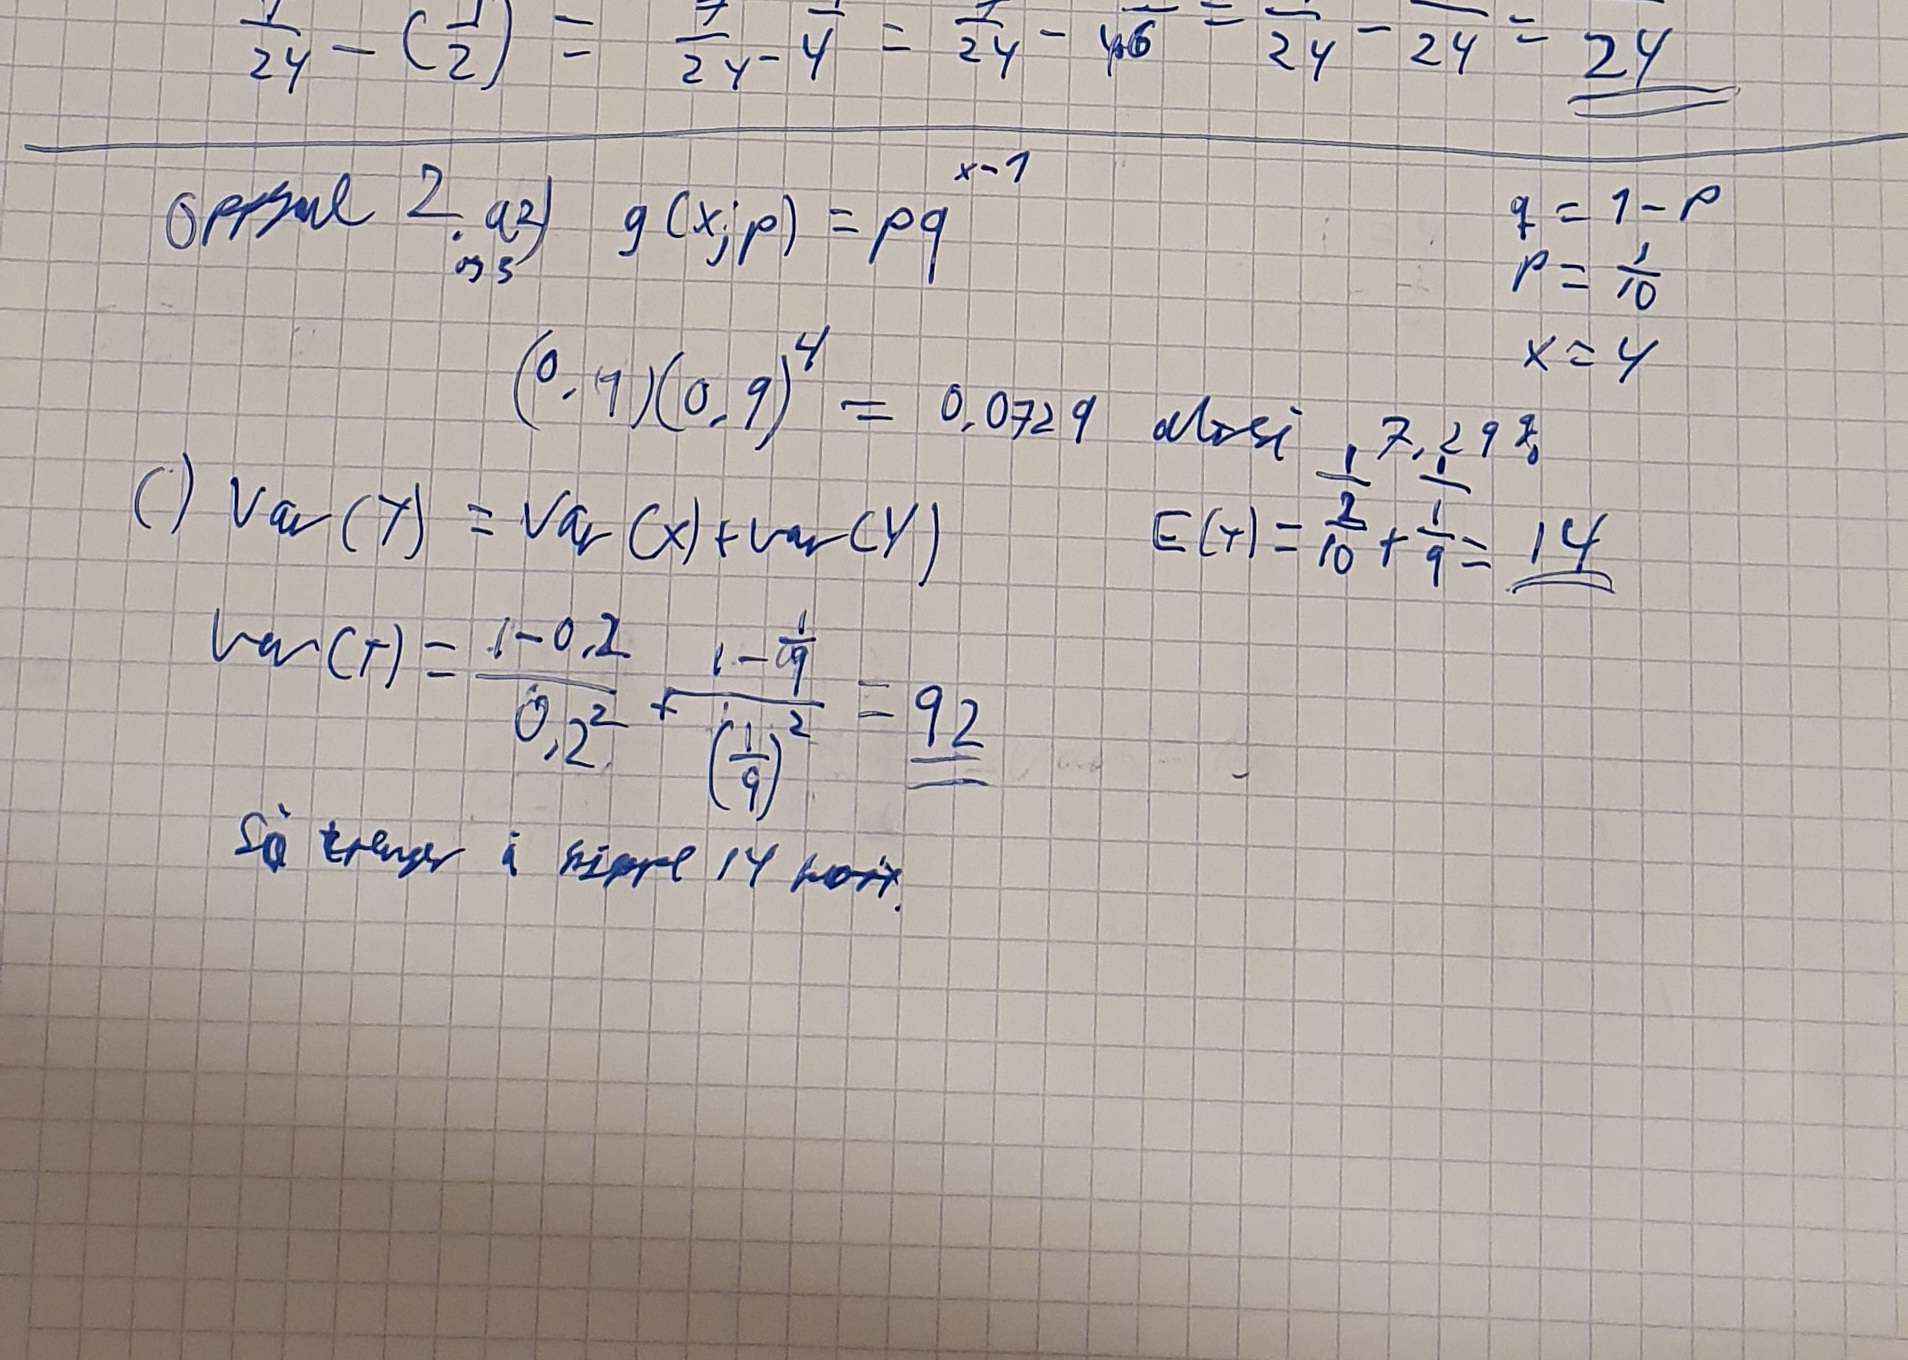
\includegraphics{oblig2_utregning/oppgave2.jpg} \clearpage

\subsection{3}\label{section-2}

Vi definerer en enhet av en råvare (kan være gull, olje, korn, etc) som
den mengden du får kjøpt for M NOK (det er ikke viktig hva M er). Du
regner med at om du kjøper en enhet av vare A blir fortjenesta etter ett
år normalfordelt med forventning \(\mu\)A = 50 NOK og standardavvik
\(\sigma\) A = 100 NOK. Vi kaller fortjenesta X:

\subsubsection{a) Om du kjøper en slik enhet av vare A hva blir
sannsynligheten
for}\label{a-om-du-kjuxf8per-en-slik-enhet-av-vare-a-hva-blir-sannsynligheten-for}

\paragraph{- at du ikke går med tap (det vil si får positiv
fortjeneste)?}\label{at-du-ikke-guxe5r-med-tap-det-vil-si-fuxe5r-positiv-fortjeneste}

\begin{Shaded}
\begin{Highlighting}[]
\ImportTok{from}\NormalTok{ scipy.stats }\ImportTok{import}\NormalTok{ norm}


\NormalTok{mu }\OperatorTok{=} \DecValTok{50}  
\NormalTok{sigma }\OperatorTok{=} \DecValTok{100}  




\DecValTok{1} \OperatorTok{{-}}\NormalTok{ norm.cdf(}\DecValTok{0}\NormalTok{, mu, sigma)}
\end{Highlighting}
\end{Shaded}

\begin{verbatim}
0.6914624612740131
\end{verbatim}

69.15\%

\paragraph{- at du ikke går med tap og at fortjenesten er mindre enn
150?}\label{at-du-ikke-guxe5r-med-tap-og-at-fortjenesten-er-mindre-enn-150}

\begin{Shaded}
\begin{Highlighting}[]
\NormalTok{norm.cdf(}\DecValTok{150}\NormalTok{, mu, sigma) }\OperatorTok{{-}}\NormalTok{ norm.cdf(}\DecValTok{0}\NormalTok{, mu, sigma)}
\end{Highlighting}
\end{Shaded}

\begin{verbatim}
0.532807207342556
\end{verbatim}

\paragraph{- at du får fortjeneste mindre enn 150, gitt at du ikke går
med
tap?}\label{at-du-fuxe5r-fortjeneste-mindre-enn-150-gitt-at-du-ikke-guxe5r-med-tap}

\begin{Shaded}
\begin{Highlighting}[]
\NormalTok{(norm.cdf(}\DecValTok{150}\NormalTok{, mu, sigma) }\OperatorTok{{-}}\NormalTok{ norm.cdf(}\DecValTok{0}\NormalTok{, mu, sigma))}\OperatorTok{/}\NormalTok{(}\DecValTok{1} \OperatorTok{{-}}\NormalTok{ norm.cdf(}\DecValTok{0}\NormalTok{, mu, sigma))}
\end{Highlighting}
\end{Shaded}

\begin{verbatim}
0.7705511682598991
\end{verbatim}

\subsubsection{b) Finn fortjenesten som er slik at du er 80\% sikker på
å få en fortjeneste over
dette.}\label{b-finn-fortjenesten-som-er-slik-at-du-er-80-sikker-puxe5-uxe5-fuxe5-en-fortjeneste-over-dette.}

\begin{Shaded}
\begin{Highlighting}[]
\NormalTok{norm.ppf(}\FloatTok{0.80}\NormalTok{)}\OperatorTok{*}\DecValTok{100}\OperatorTok{+}\DecValTok{50}
\end{Highlighting}
\end{Shaded}

\begin{verbatim}
134.16212335729142
\end{verbatim}

(I oppgave c) er fortsatt standardavviket 100 NOK.)

\subsubsection{c) Hva må forventningsverdien være for å ha en
sannsynlighet på 90\% for ikke å gå med
tap}\label{c-hva-muxe5-forventningsverdien-vuxe6re-for-uxe5-ha-en-sannsynlighet-puxe5-90-for-ikke-uxe5-guxe5-med-tap}

\begin{Shaded}
\begin{Highlighting}[]
\NormalTok{norm.ppf(}\FloatTok{0.9}\NormalTok{)}\OperatorTok{*}\DecValTok{100}
\end{Highlighting}
\end{Shaded}

\begin{verbatim}
128.15515655446004
\end{verbatim}

\clearpage

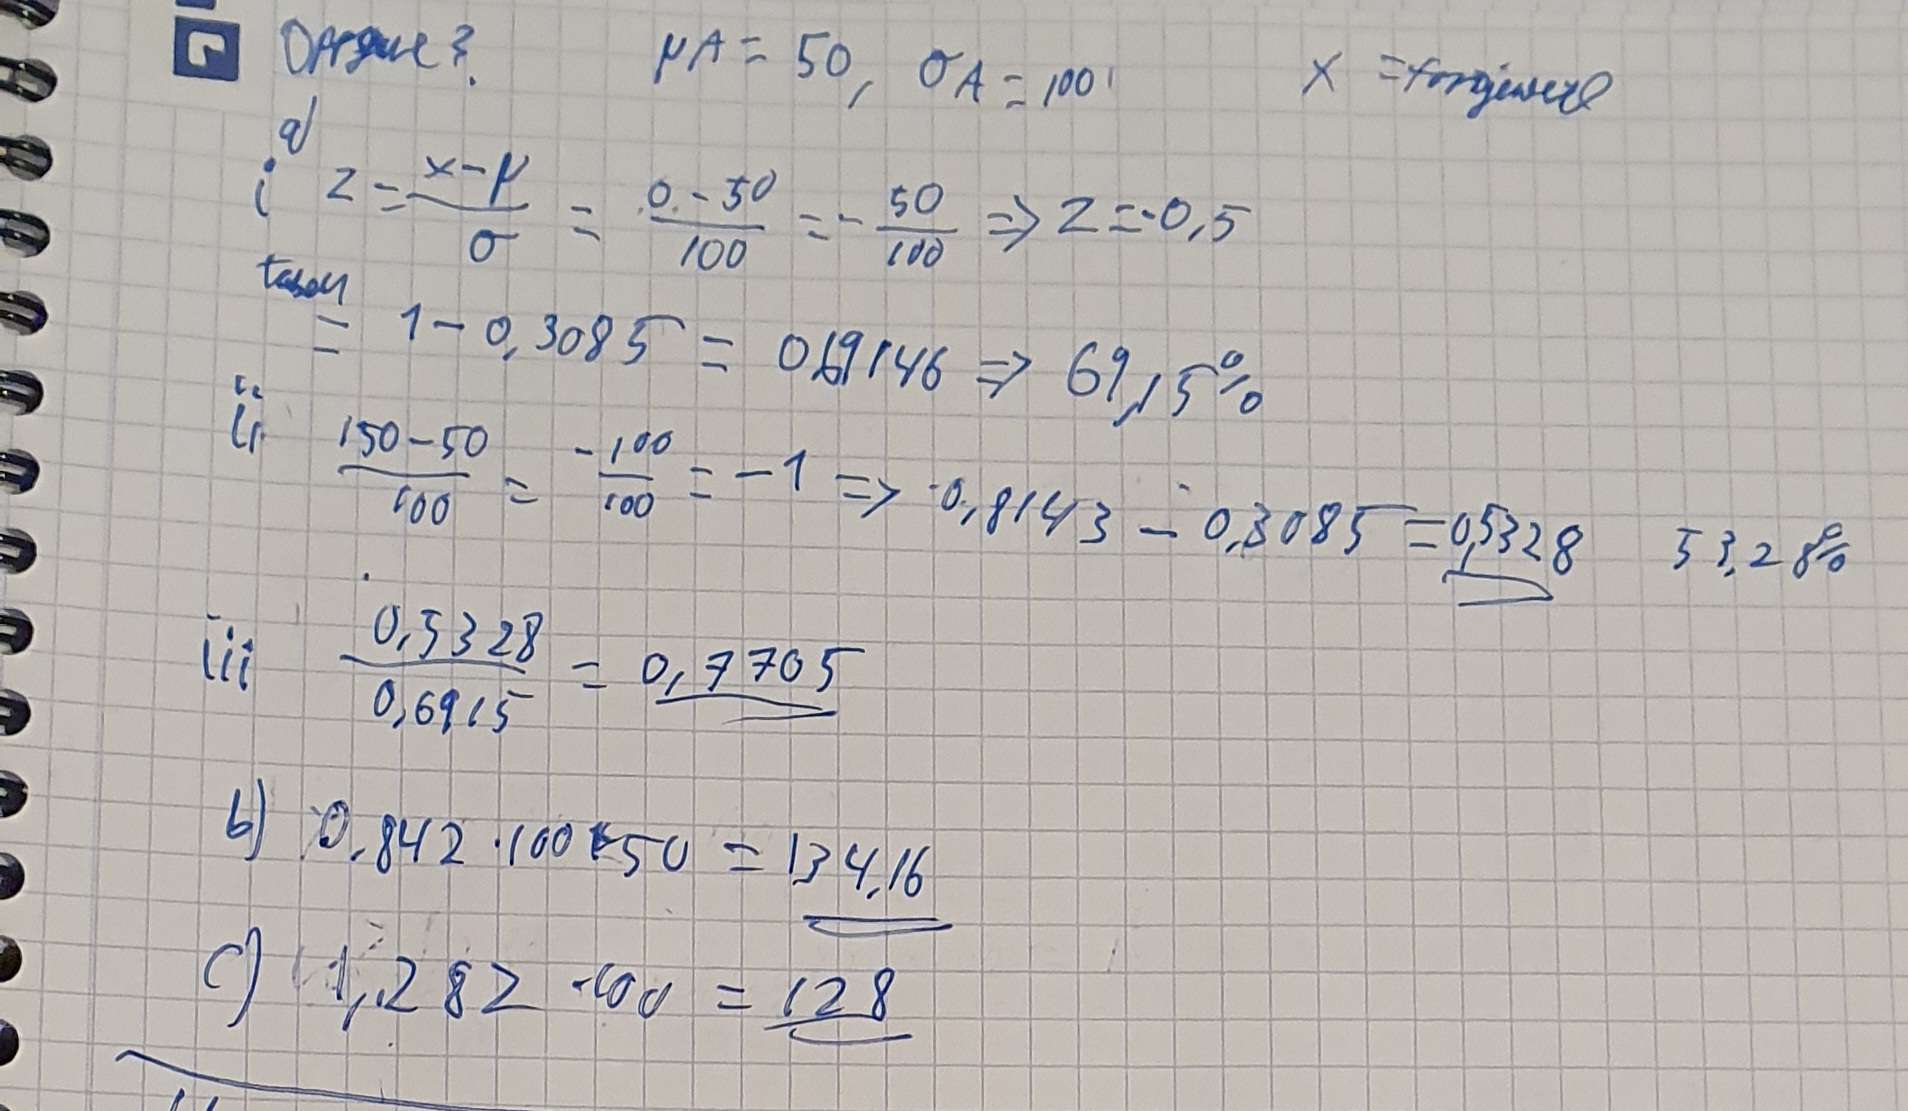
\includegraphics{oblig2_utregning/oppgave3.jpg}

\clearpage

\subsection{4}\label{section-3}

Har brukt tiden min dårlig så når ikke å gjøre denne oppgaven før
fristen

Vi definerer igjen en enhet av en vare som den mengden du får kjøpt for
M NOK. Nå vil du kjøpe to varer, vare A og vare B, og du regner med at
fortjenestene for en enhet etter ett år er respektive

\[ 
X ∼ N(\mu A, \sigma A) \> \> \> \> \> \text{og} \> \> \> \> \> Y ∼ N(\mu B , \sigma B )
\] Vi antar og at X og Y er uavhengige

Vi vil se på total fortjeneste etter ett år om du til sammen har kjøpt
for beløpet M , men bruker 30\% på vare A og 70\% på vare B, altså total
fortjeneste gitt ved:

\[
T = 0.3 · X + 0.7 · Y
\]

I oppgave a) og b) går vi ut fra at \(\mu\)A = 50, \(\mu\)B = 50,
\(\sigma\)A = 100 og \(\sigma\)B = 50.

\subsubsection{a) Finn forventningsverdien og variansen til den totale
fortjenesta.}\label{a-finn-forventningsverdien-og-variansen-til-den-totale-fortjenesta.}

Hva blir fordelinga til den totale fortjenesta?

\subsubsection{b) Bruk fordelinga fra a) til å finne et 95\%
prediksjonsintervall for den totale
fortjenesta.}\label{b-bruk-fordelinga-fra-a-til-uxe5-finne-et-95-prediksjonsintervall-for-den-totale-fortjenesta.}

Nå går vi ut fra at du vil kjøpe varer av type A og B slik at total
forjeneste blir \[
T = aX + bY,
\] der \(a + b = 1\) og a og b er ikke-negative.

Du ønsker å finne hva a (og b) må være for at variansen i fortjenesta
skal bli minst mulig.

\subsubsection{c) Hva blir uttrykket for variansen til T
?}\label{c-hva-blir-uttrykket-for-variansen-til-t}

Hva er den verdien av a (uttrykt ved \(\sigma\)A og \(\sigma\)B ) som
gjør variansen for fortjenesta minst mulig? Hva blir variansen til
fortjenesta (uttrykt ved \(\sigma\)A og \(\sigma\)B ) med denne verdian
for A?

Frivillig: Anta igjen \(\sigma\)A = 100, \(\sigma\)B = 50, og lag en
figur for variansen til T som funksjon av a.



\end{document}
